\begin{figure}[h]
	\begin{minipage}{0.48\linewidth}
		\centering
		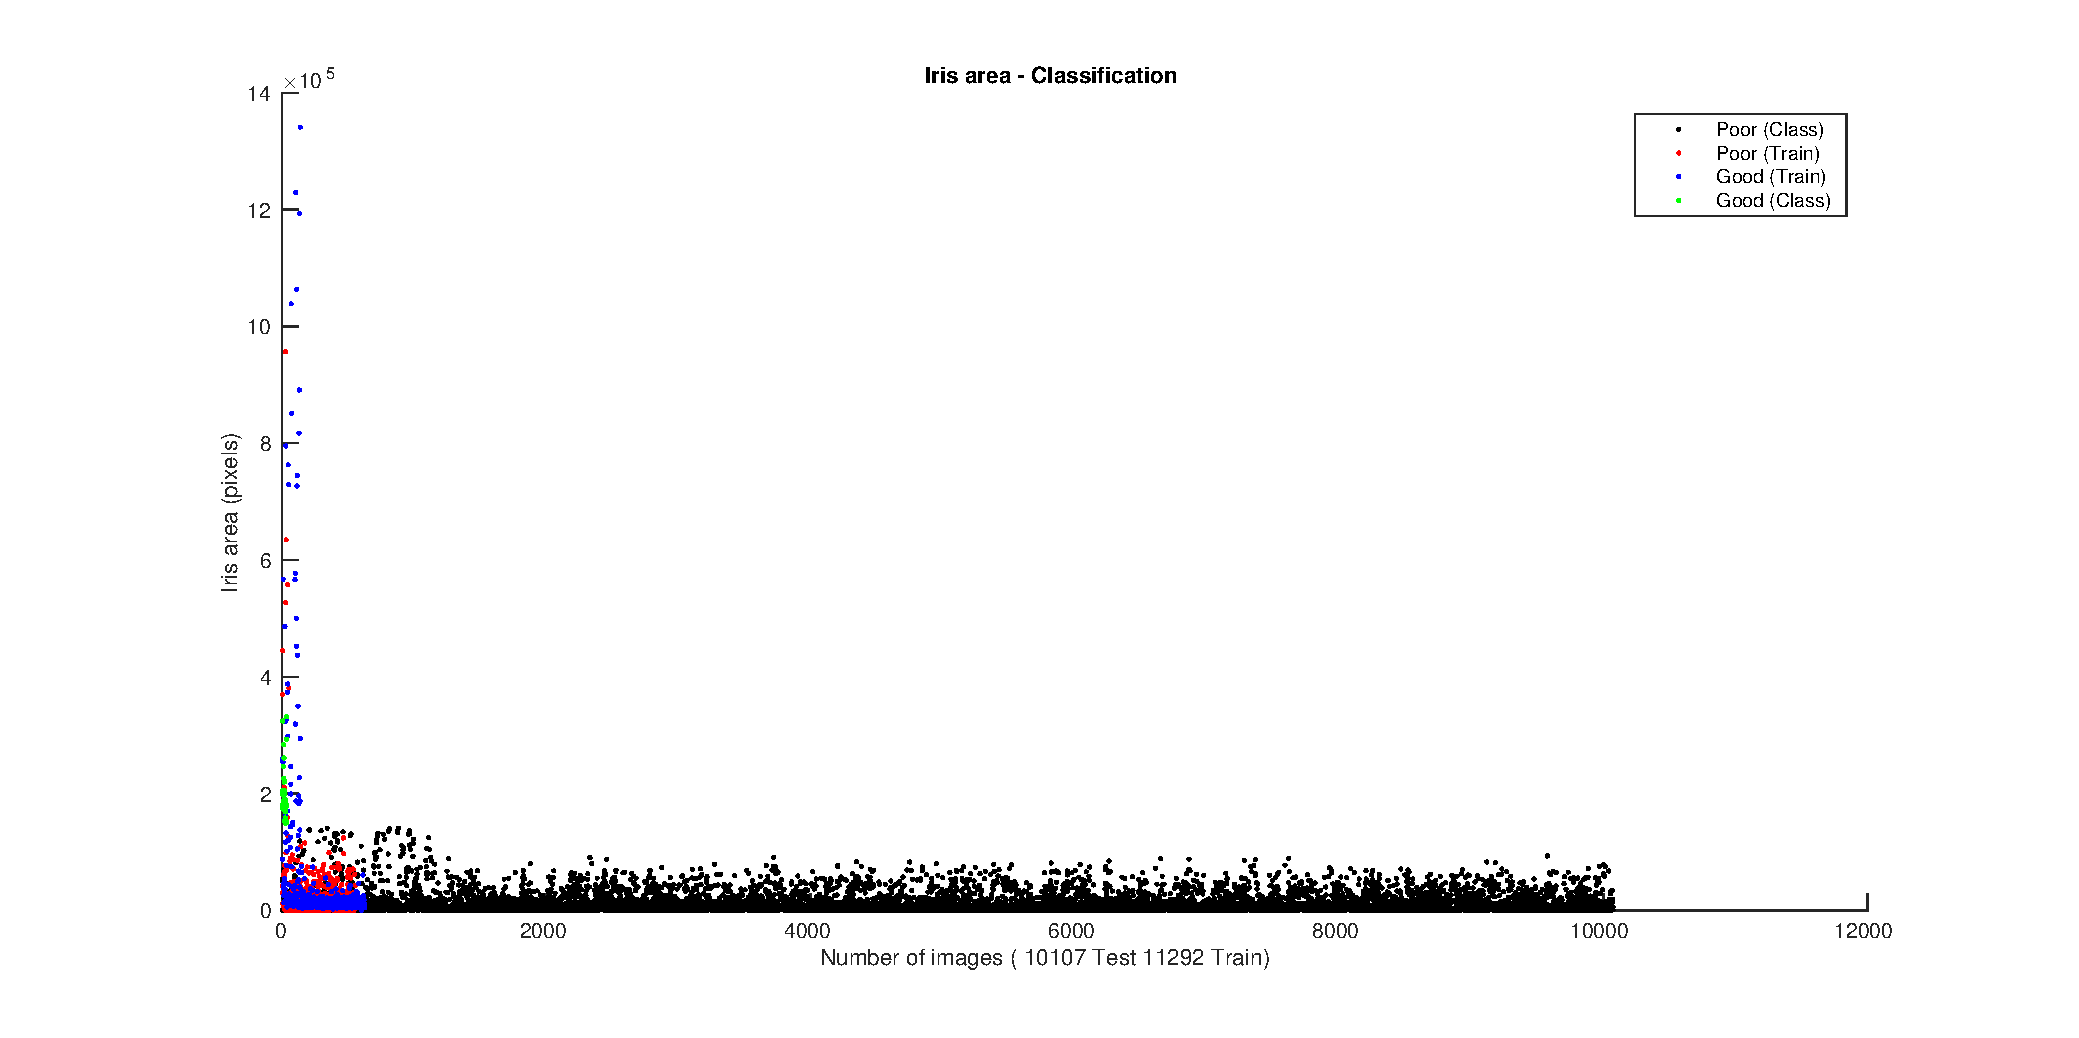
\includegraphics[width=0.9\linewidth, height=1.6cm]{pics/iqa_clas_area}
		\caption{Res. of class. using IQA iris area}
		\label{fig:clas_ia}
	\end{minipage}
	\hfill
	\begin{minipage}{0.48\linewidth}
		\centering
		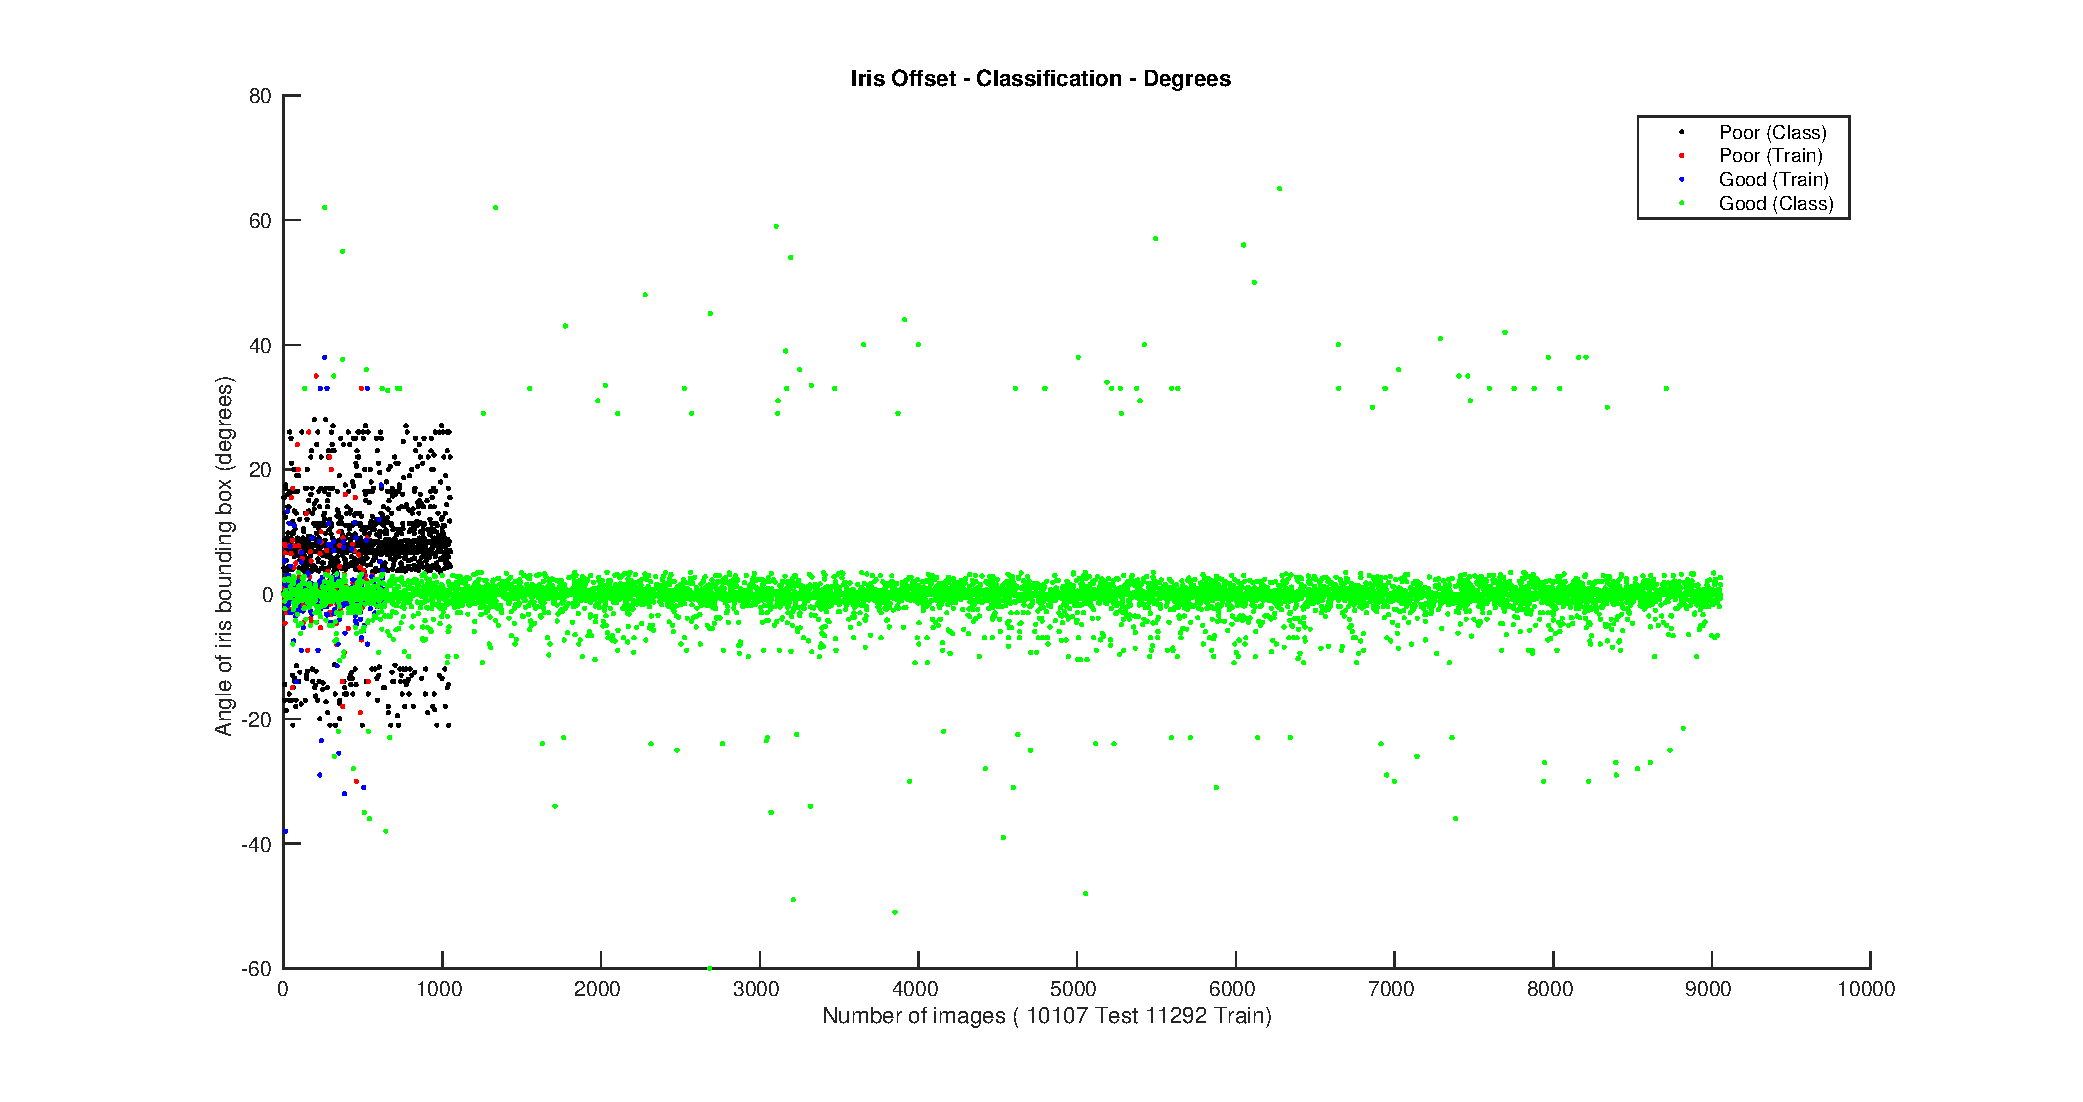
\includegraphics[width=0.9\linewidth, height=1.6cm]{pics/iqa_clas_iris_angle}
		\caption{Res. of class. using IQA iris angle}
		\label{fig:clas_ang}
	\end{minipage}
	\begin{minipage}{0.48\linewidth}
		\centering
		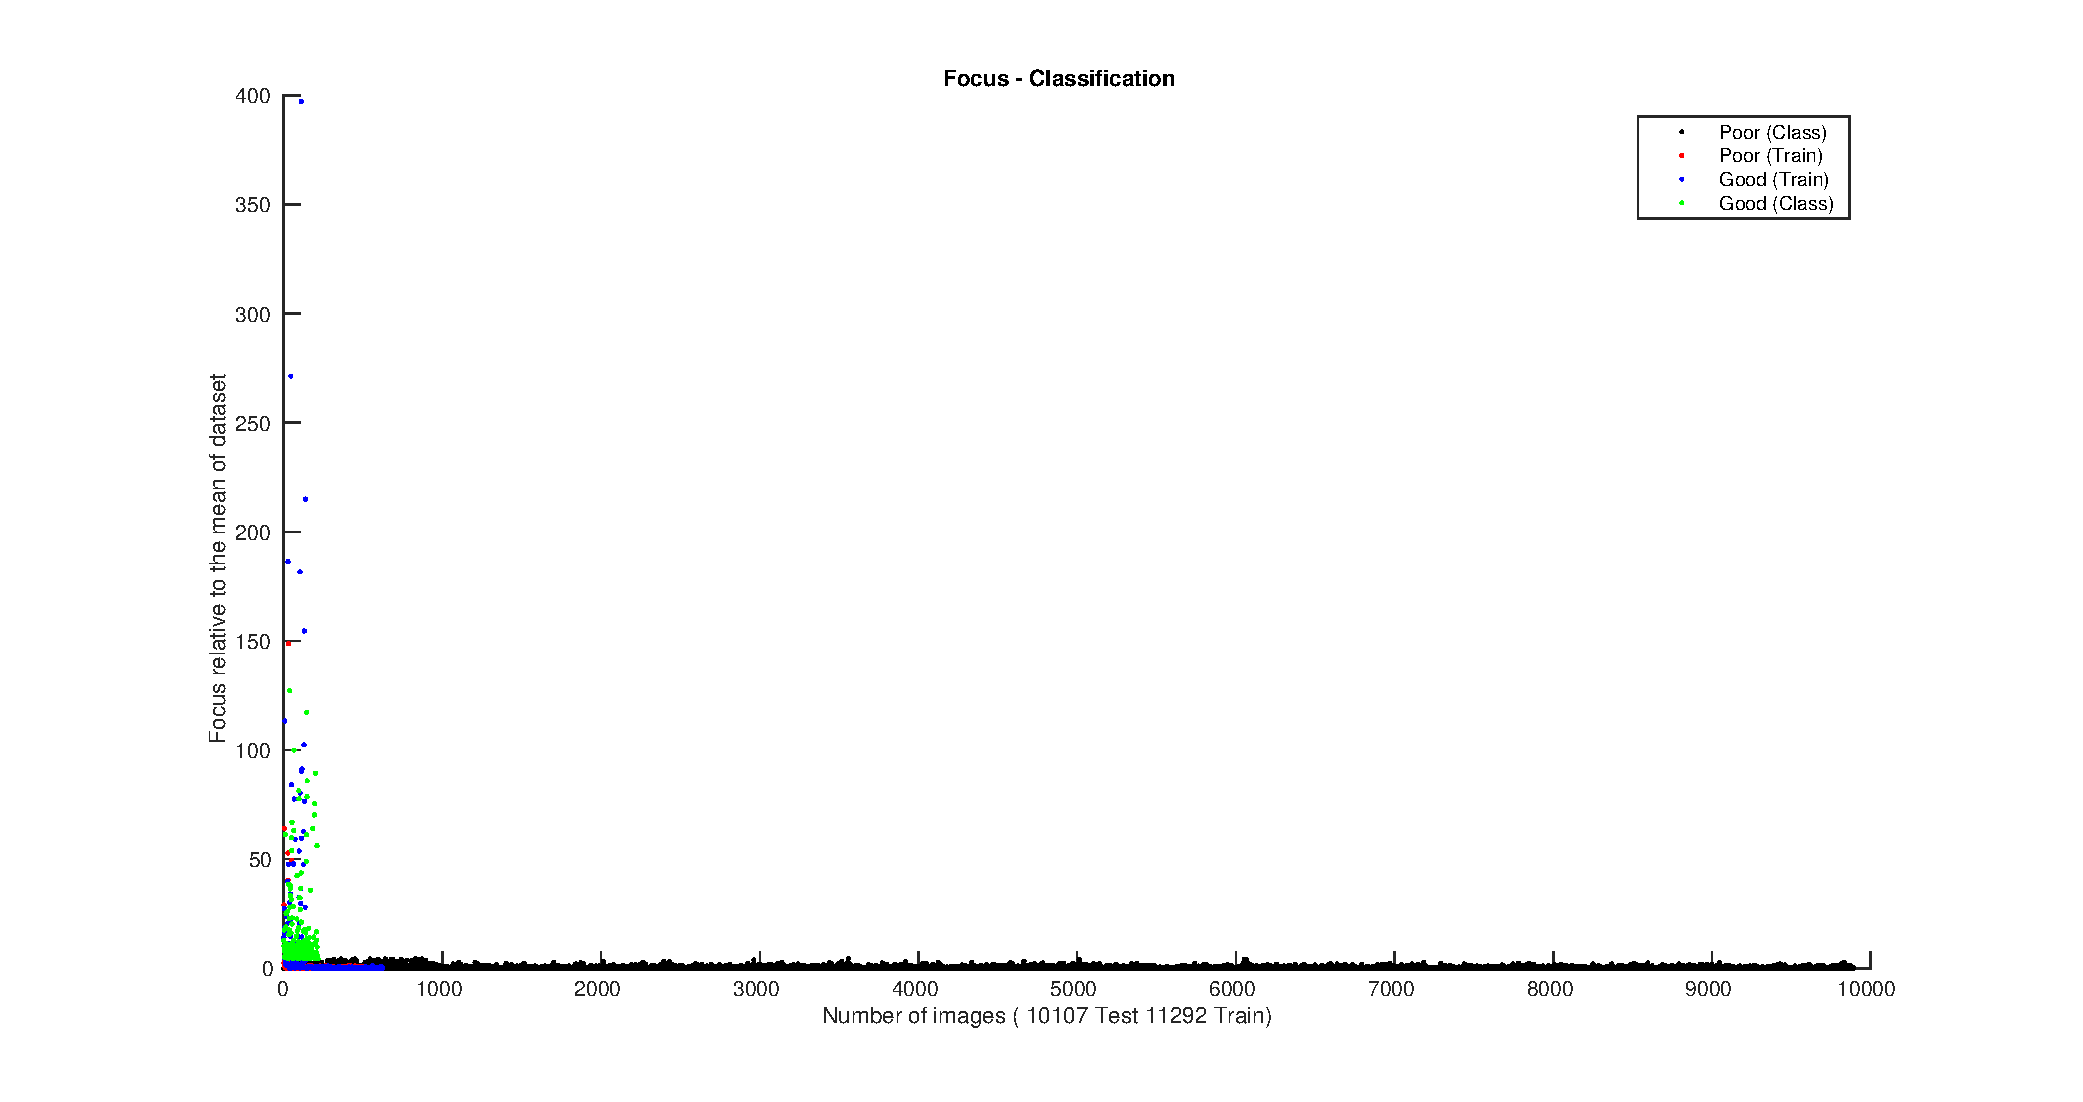
\includegraphics[width=0.9\linewidth, height=1.6cm]{pics/iqa_clas_focus}
		\caption{Res. of class. using IQA focus}
		\label{fig:clas_f}
	\end{minipage}
	\hfill
	\begin{minipage}{0.48\linewidth}
		\centering
		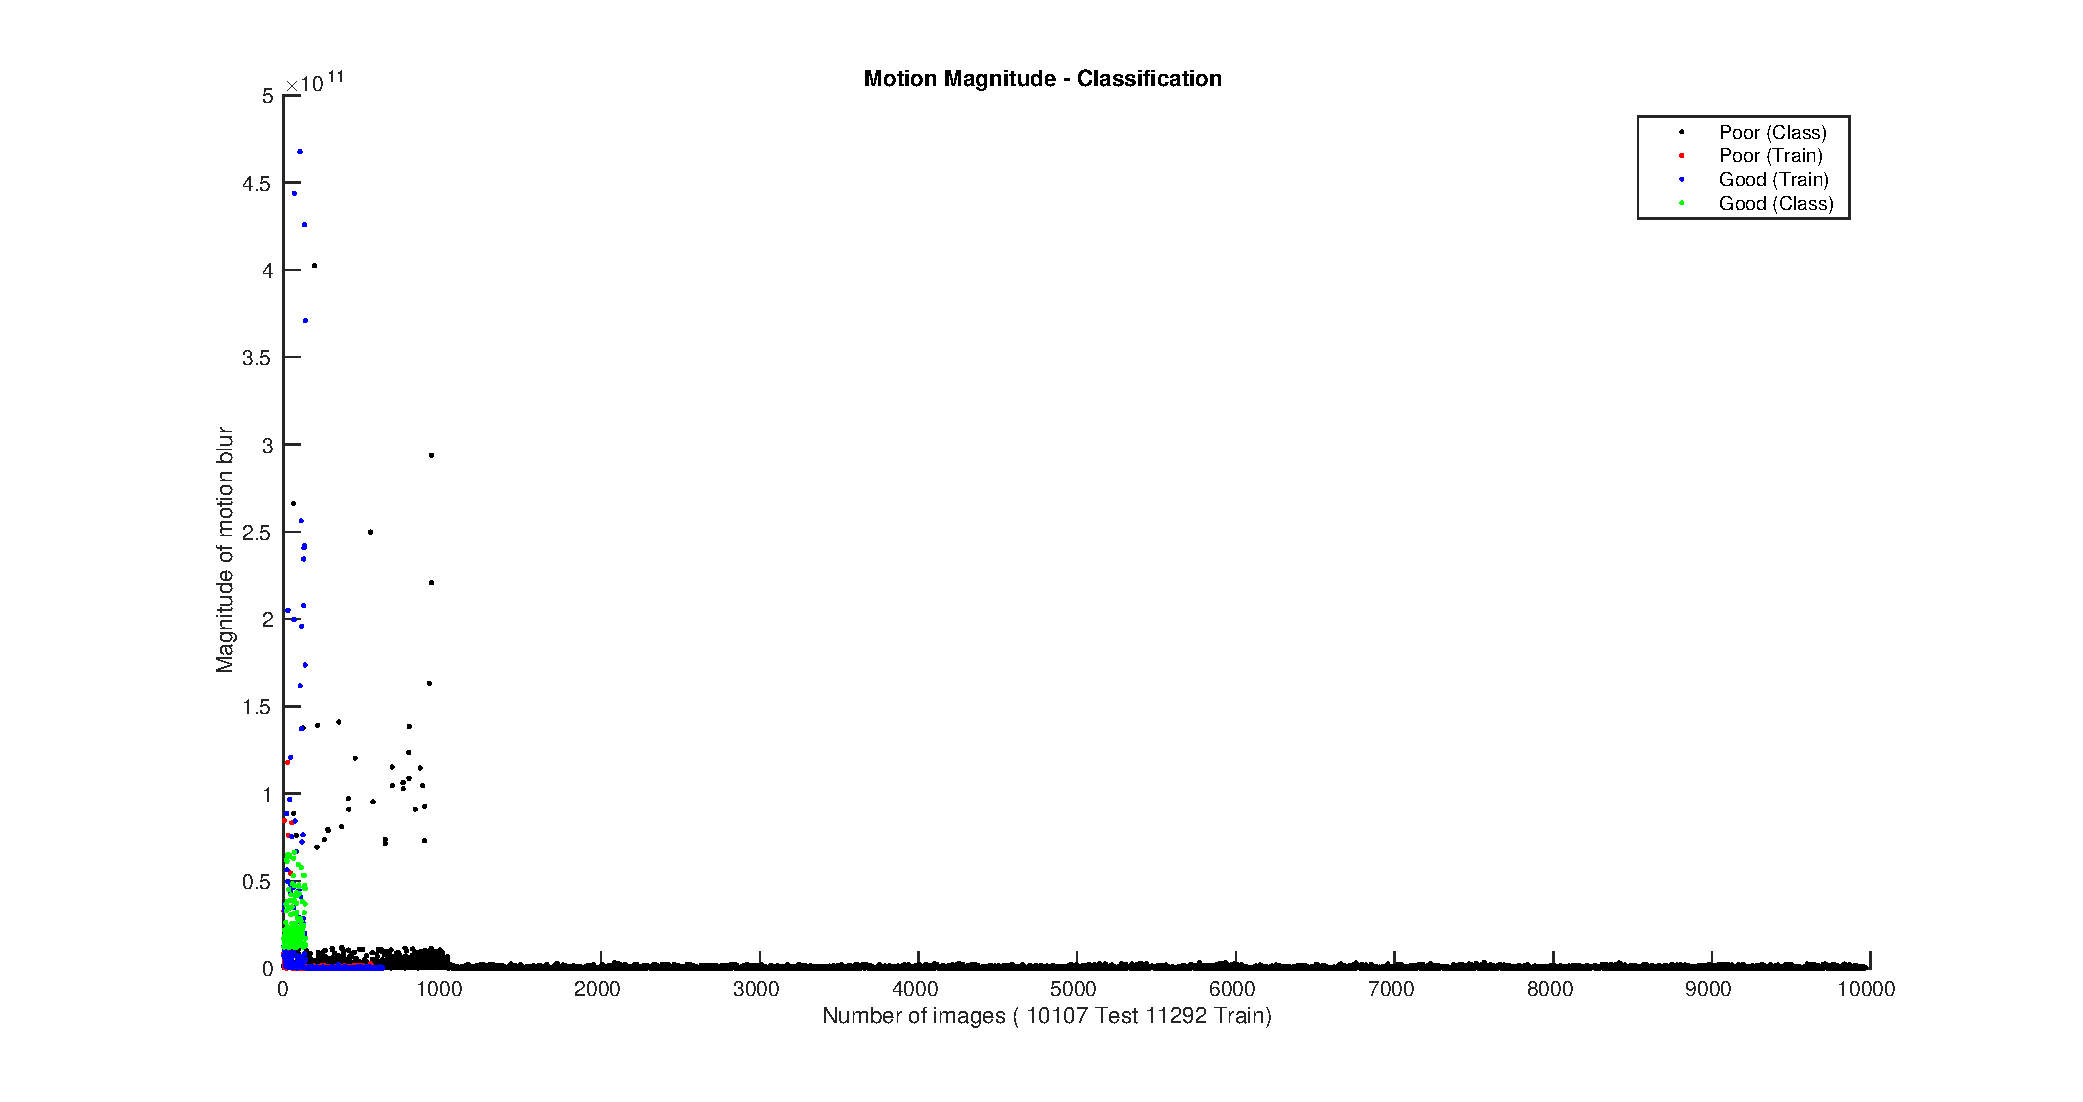
\includegraphics[width=0.9\linewidth, height=1.6cm]{pics/iqa_clas_motion}
		\caption{Res. of class. using IQA motion}
		\label{fig:clas_mot}
	\end{minipage}
	\begin{minipage}{0.48\linewidth}
		\centering
		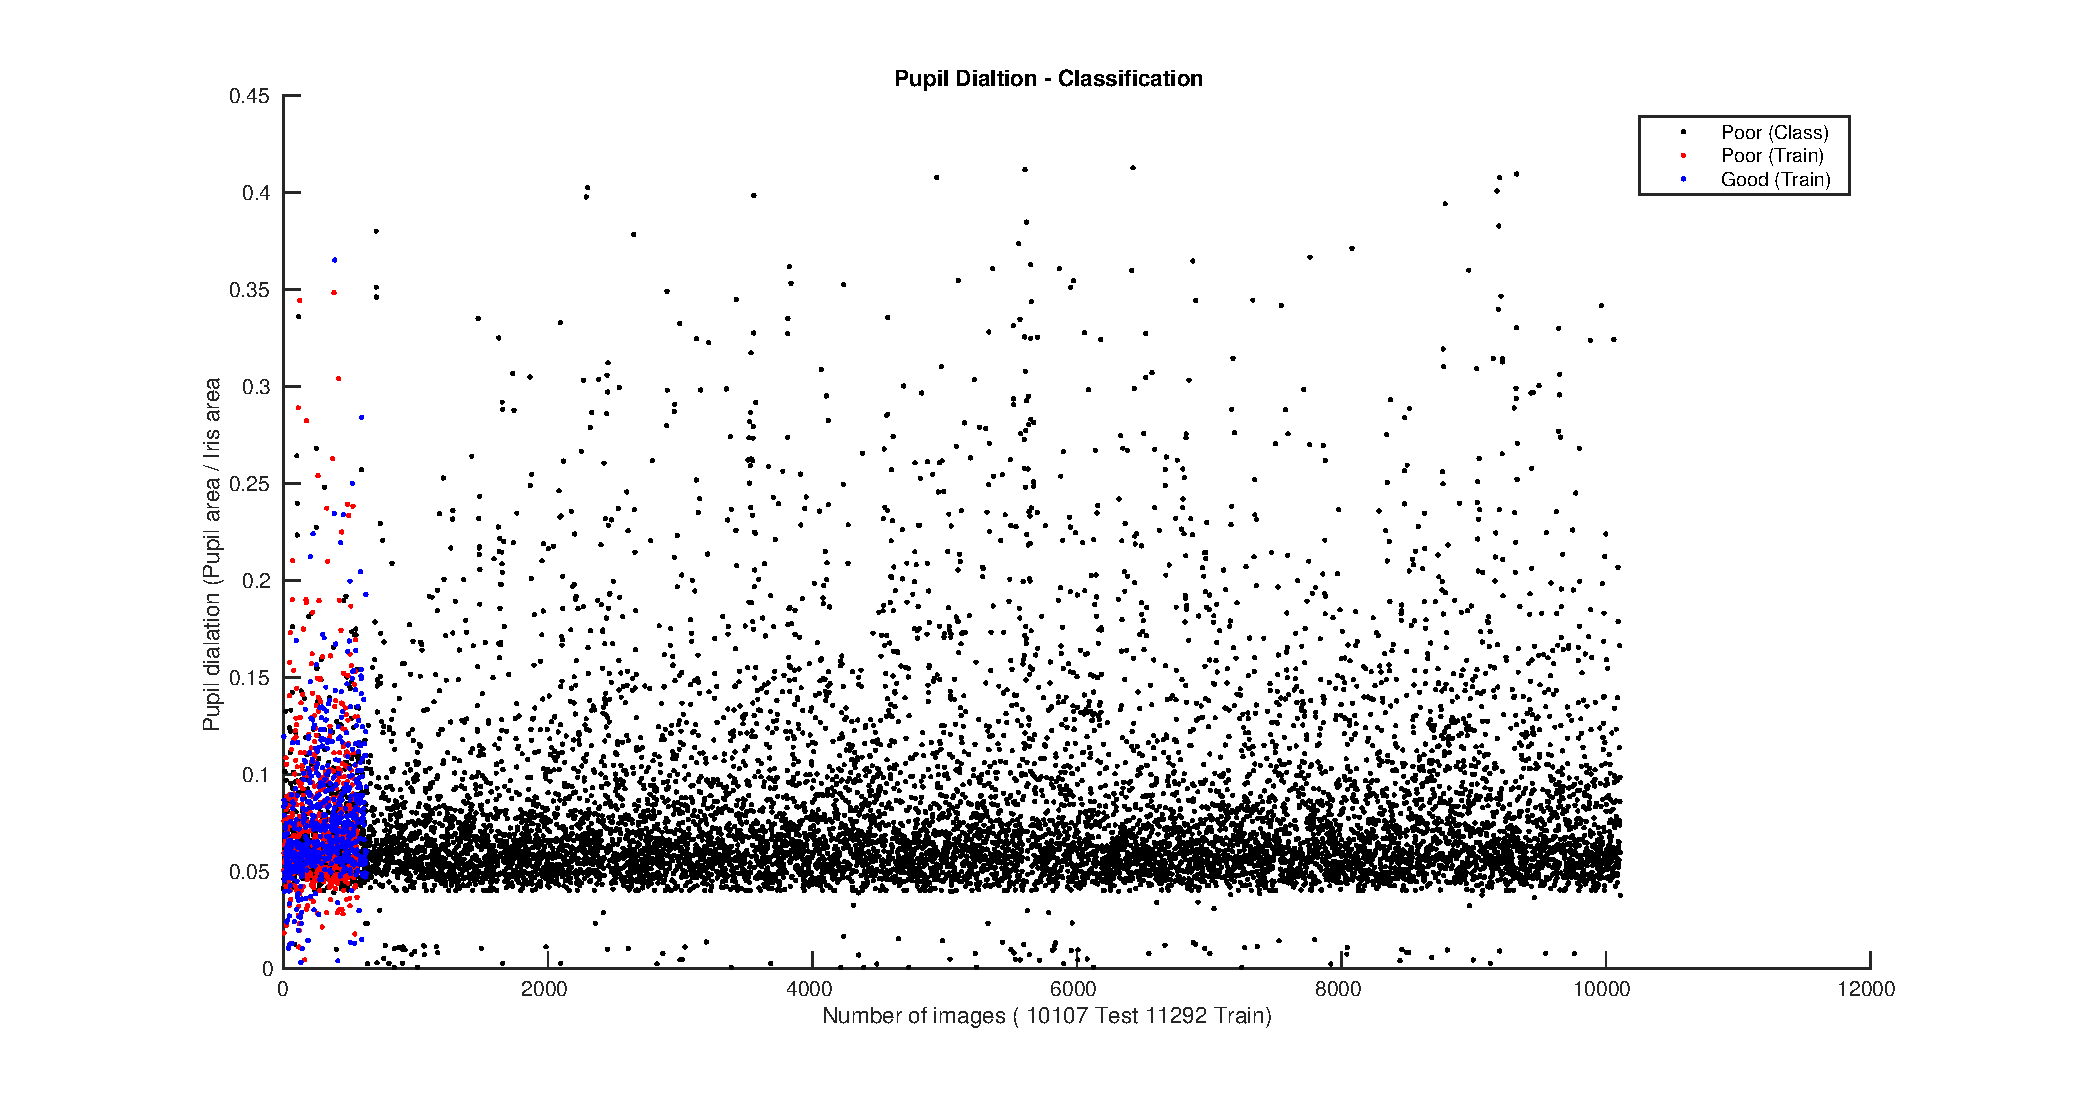
\includegraphics[width=0.9\linewidth, height=1.6cm]{pics/iqa_clas_pup_dial}
		\caption{Res. of class. using IQA pupil dilation}
		\label{fig:clas_pd}
	\end{minipage}
	\hfill
	\begin{minipage}{0.48\linewidth}
		\centering
		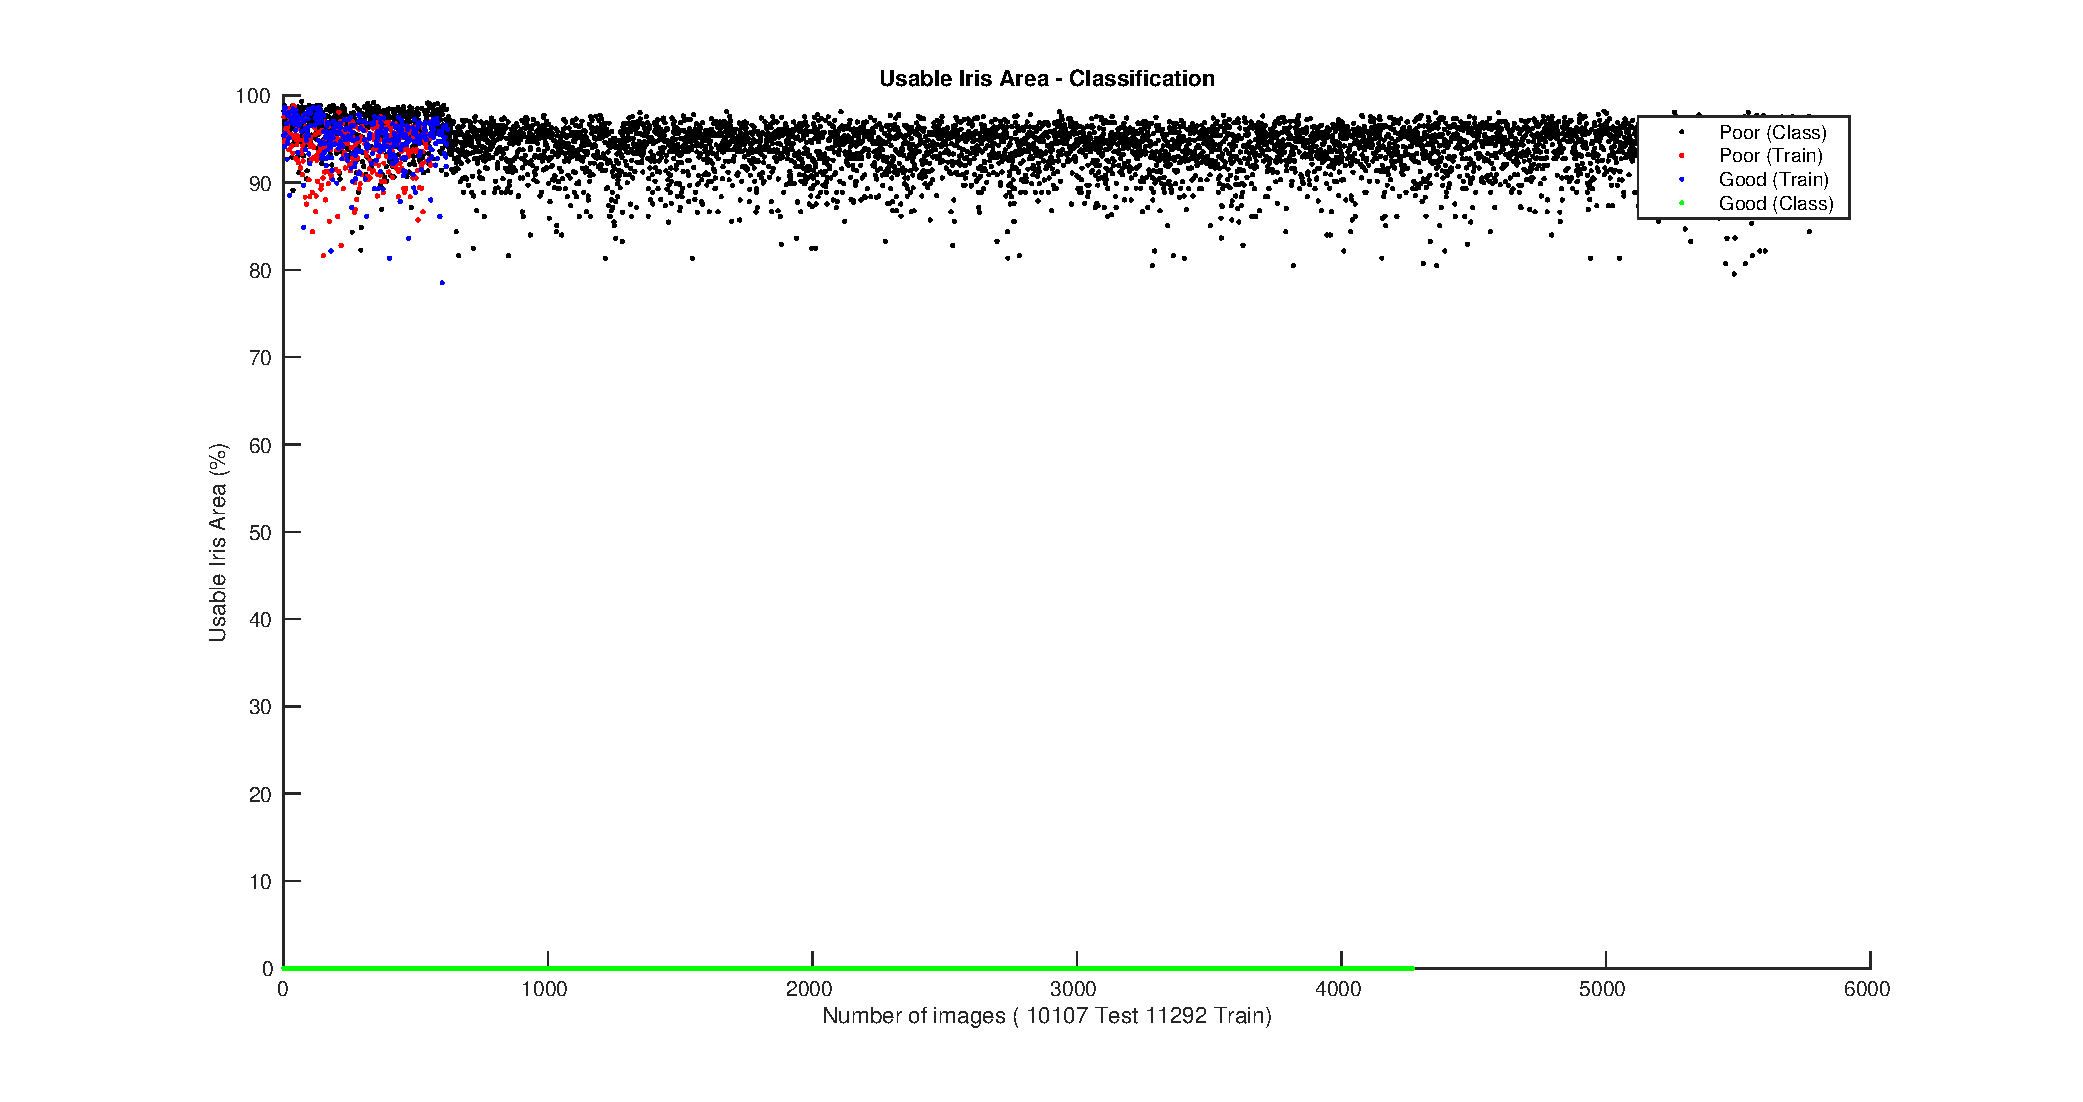
\includegraphics[width=0.9\linewidth, height=1.6cm]{pics/iqa_clas_usable_area}
		\caption{Res. of class. using BIQA UIA}
		\label{fig:clas_ua}
	\end{minipage}
	\begin{minipage}{0.48\linewidth}
		\centering
		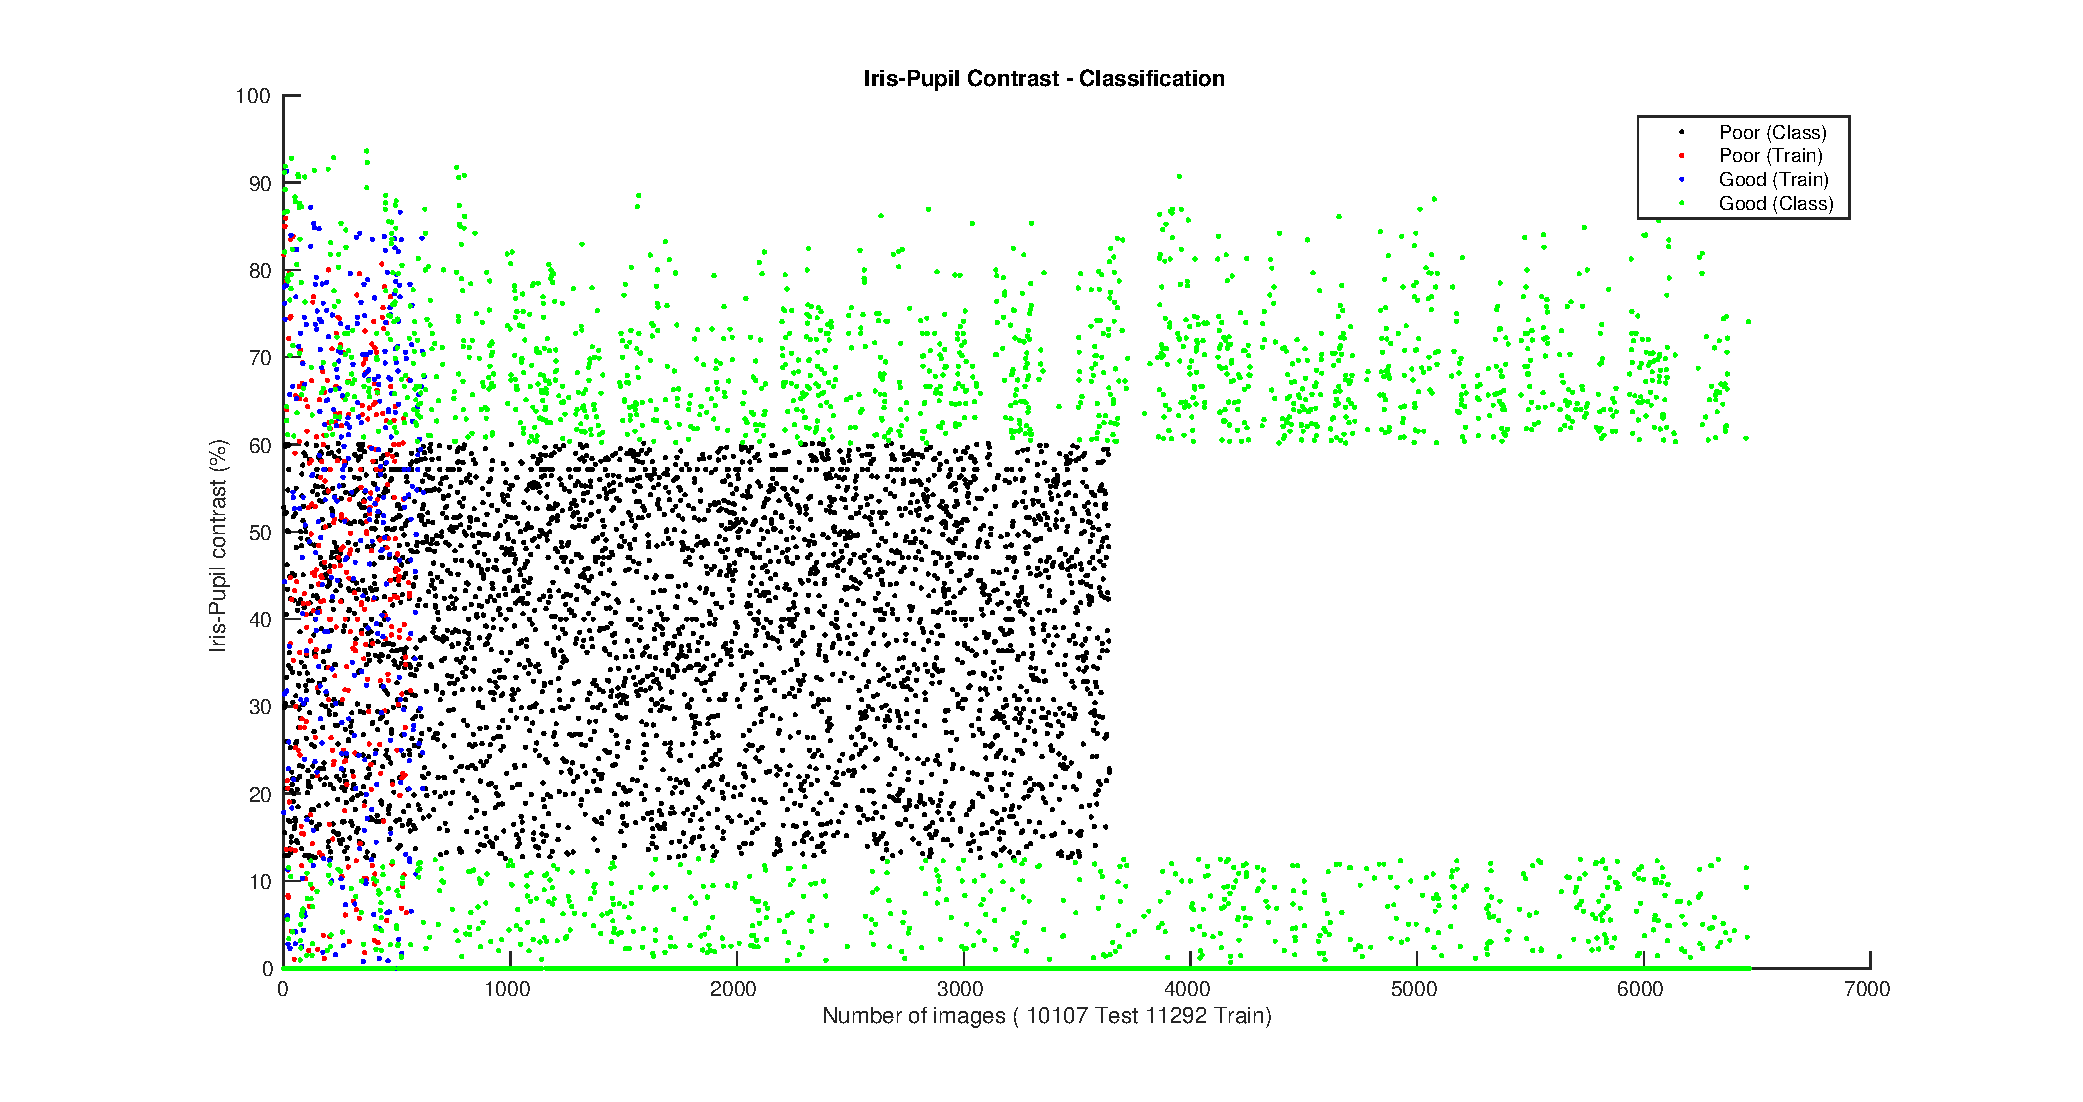
\includegraphics[width=0.9\linewidth, height=1.6cm]{pics/biqa_clas_ipc}
		\caption{Res. of class. using BIQA IPC}
		\label{fig:clas_ipc}
	\end{minipage}
	\hfill
	\begin{minipage}{0.48\linewidth}
		\centering
		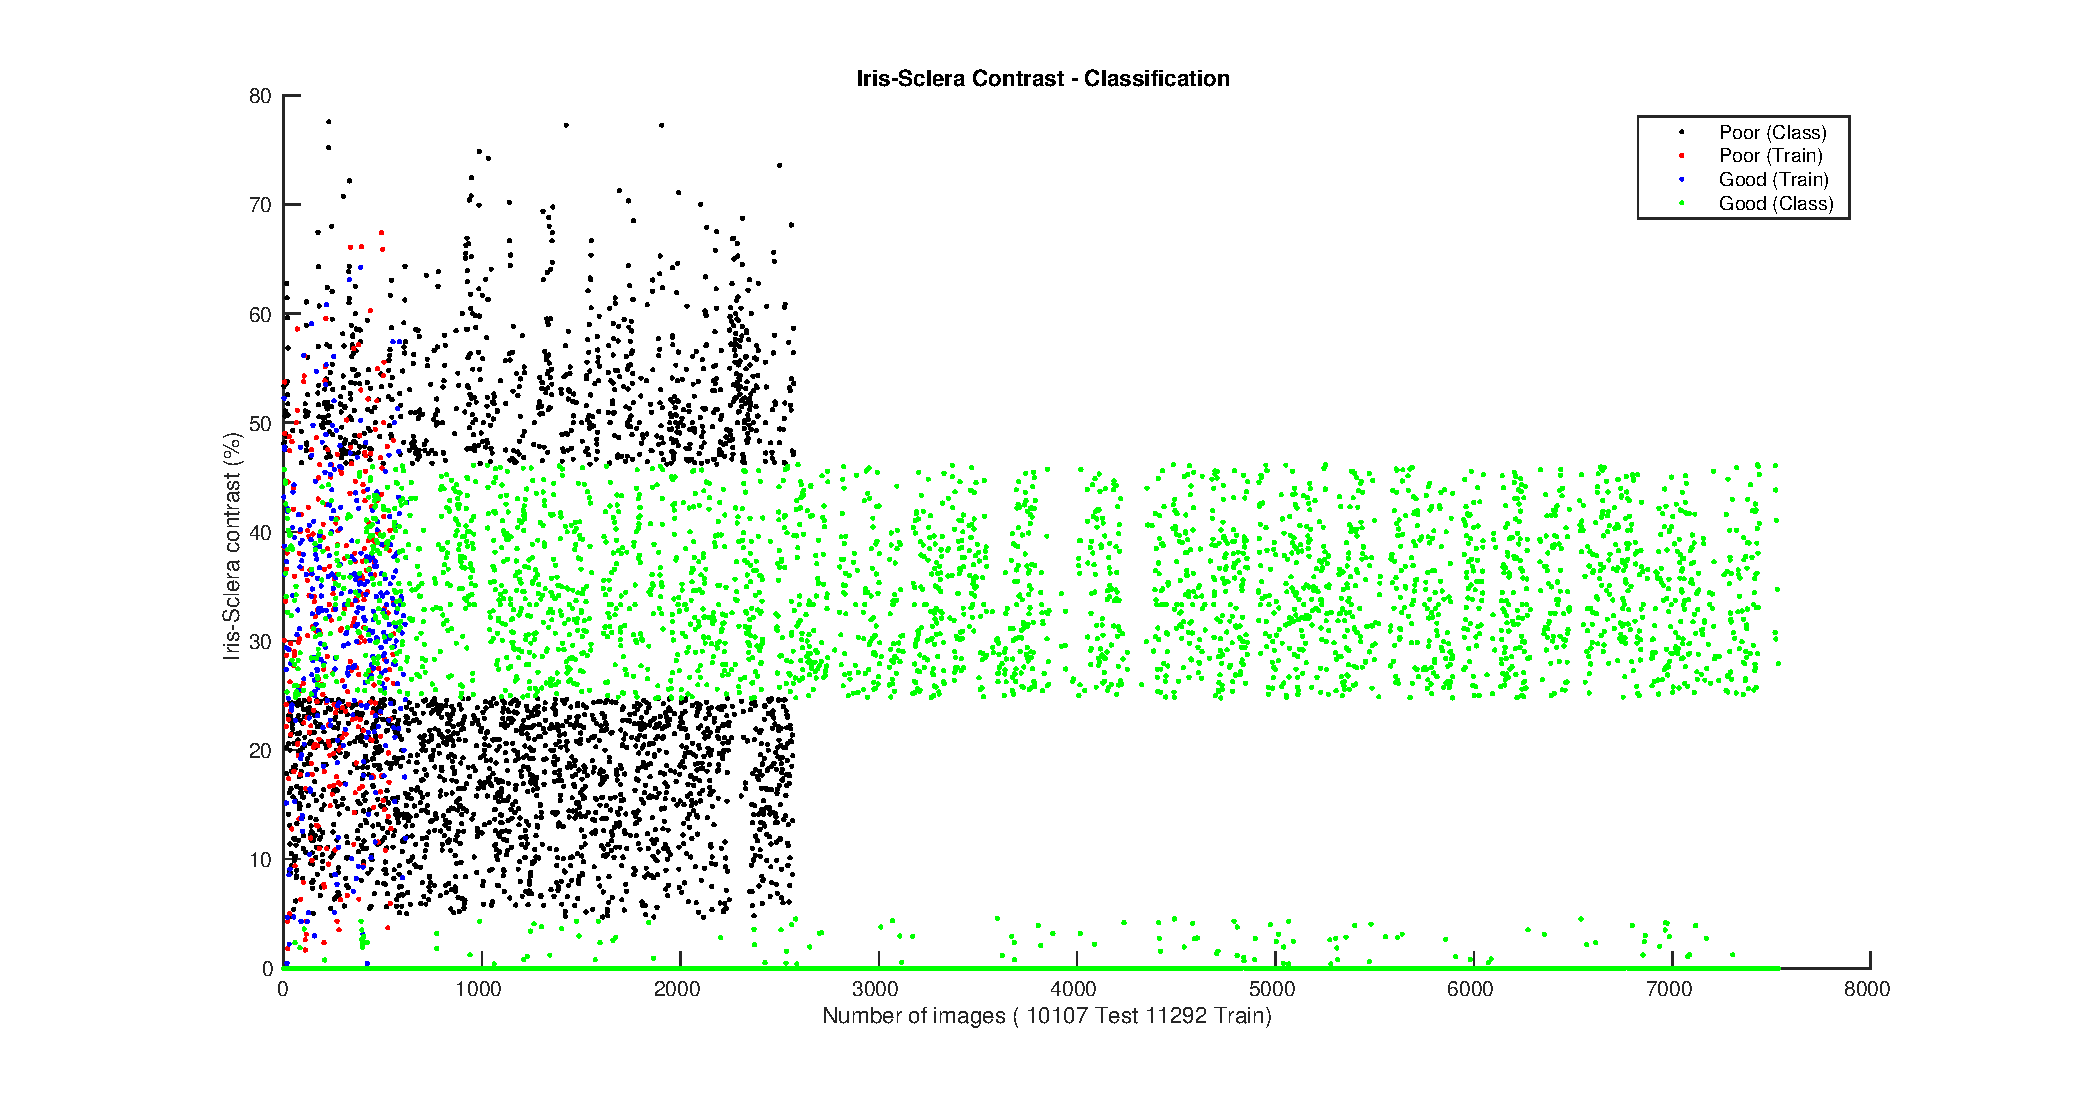
\includegraphics[width=0.9\linewidth, height=1.6cm]{pics/biqa_clas_isc}
		\caption{Res. of class. using BIQA ISC}
		\label{fig:clas_isc}
	\end{minipage}
	\begin{minipage}{0.48\linewidth}
		\centering
		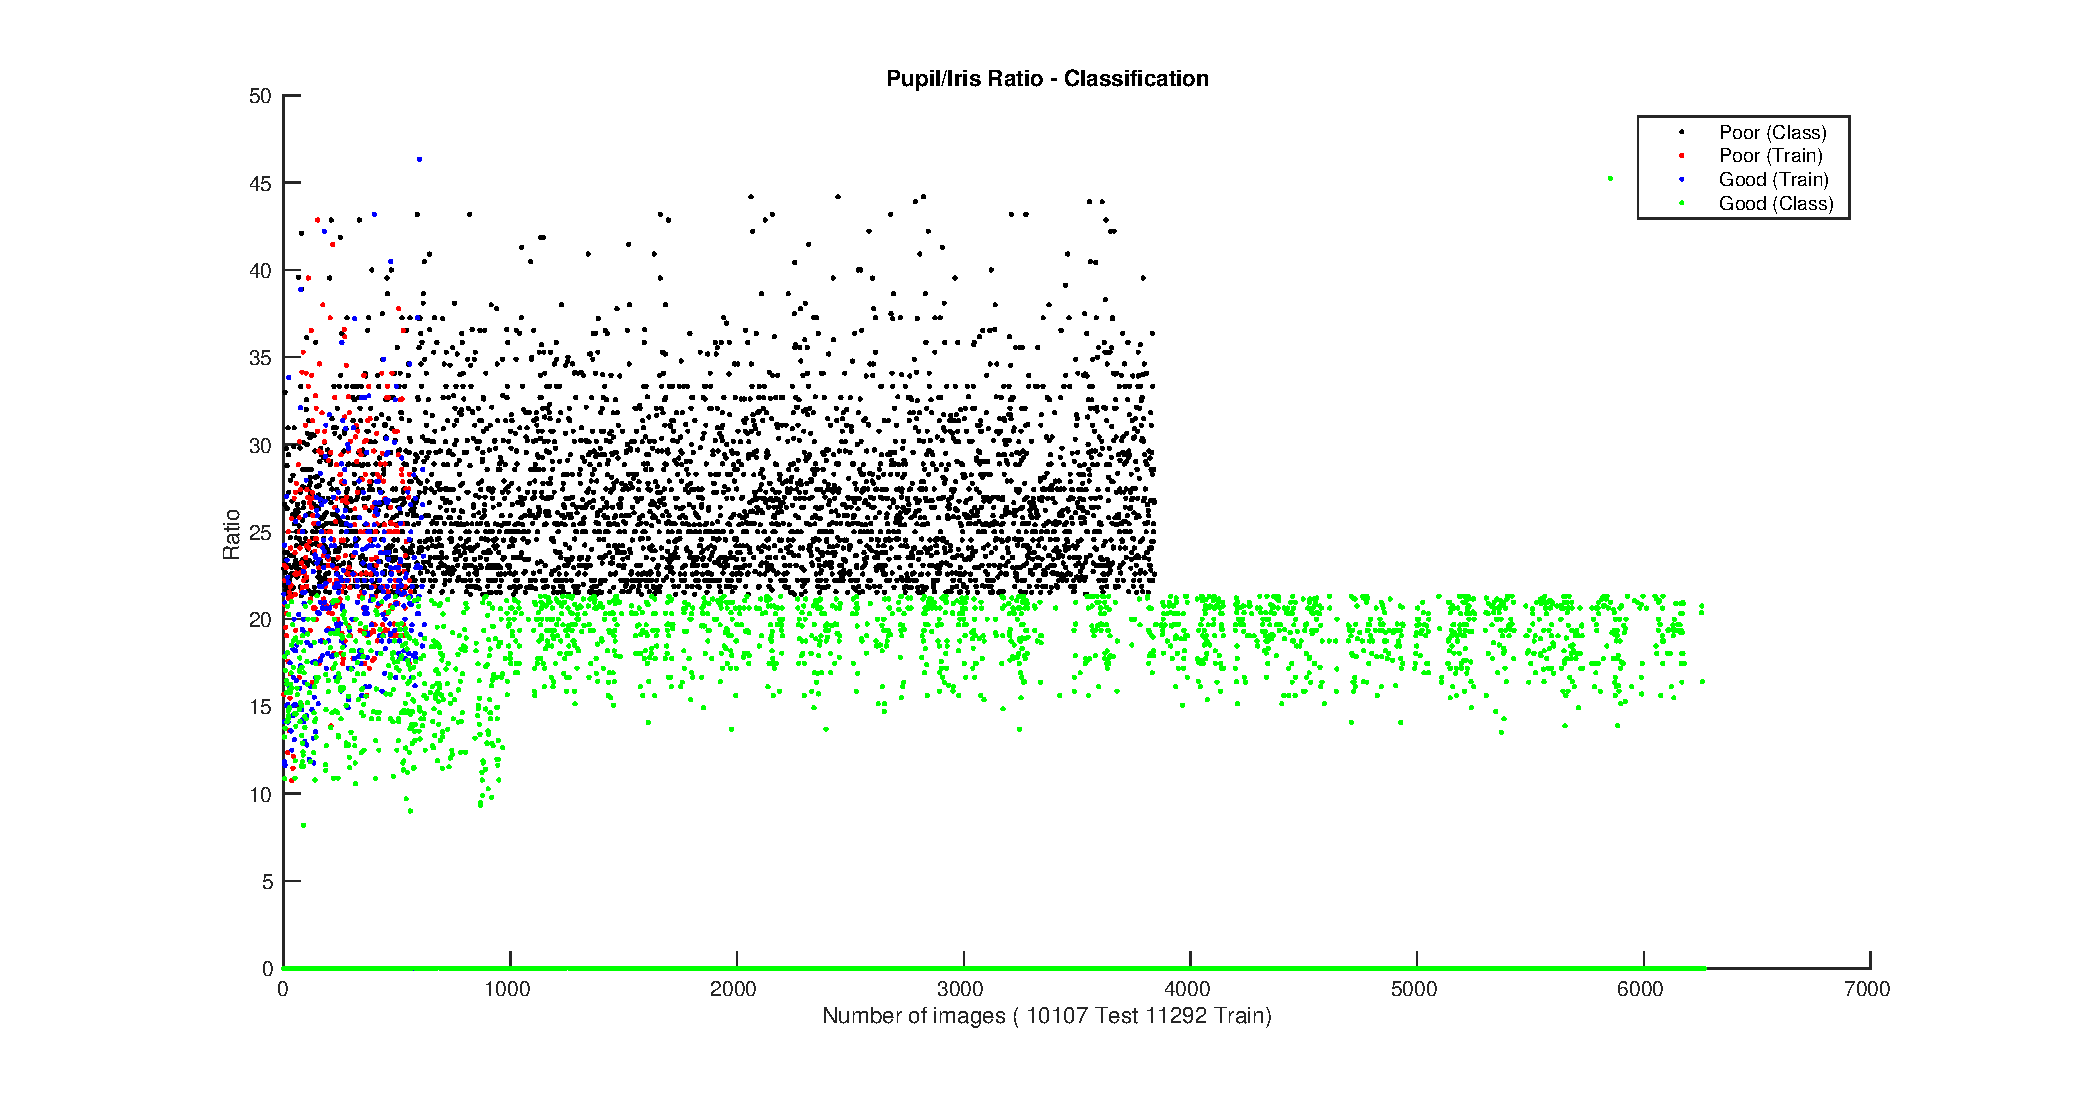
\includegraphics[width=0.9\linewidth, height=1.6cm]{pics/biqa_clas_pir}
		\caption{Res. of class. using BIQA pupil-iris rat.}
		\label{fig:clas_pir}
	\end{minipage}
	\hfill
	\begin{minipage}{0.48\linewidth}
		\centering
		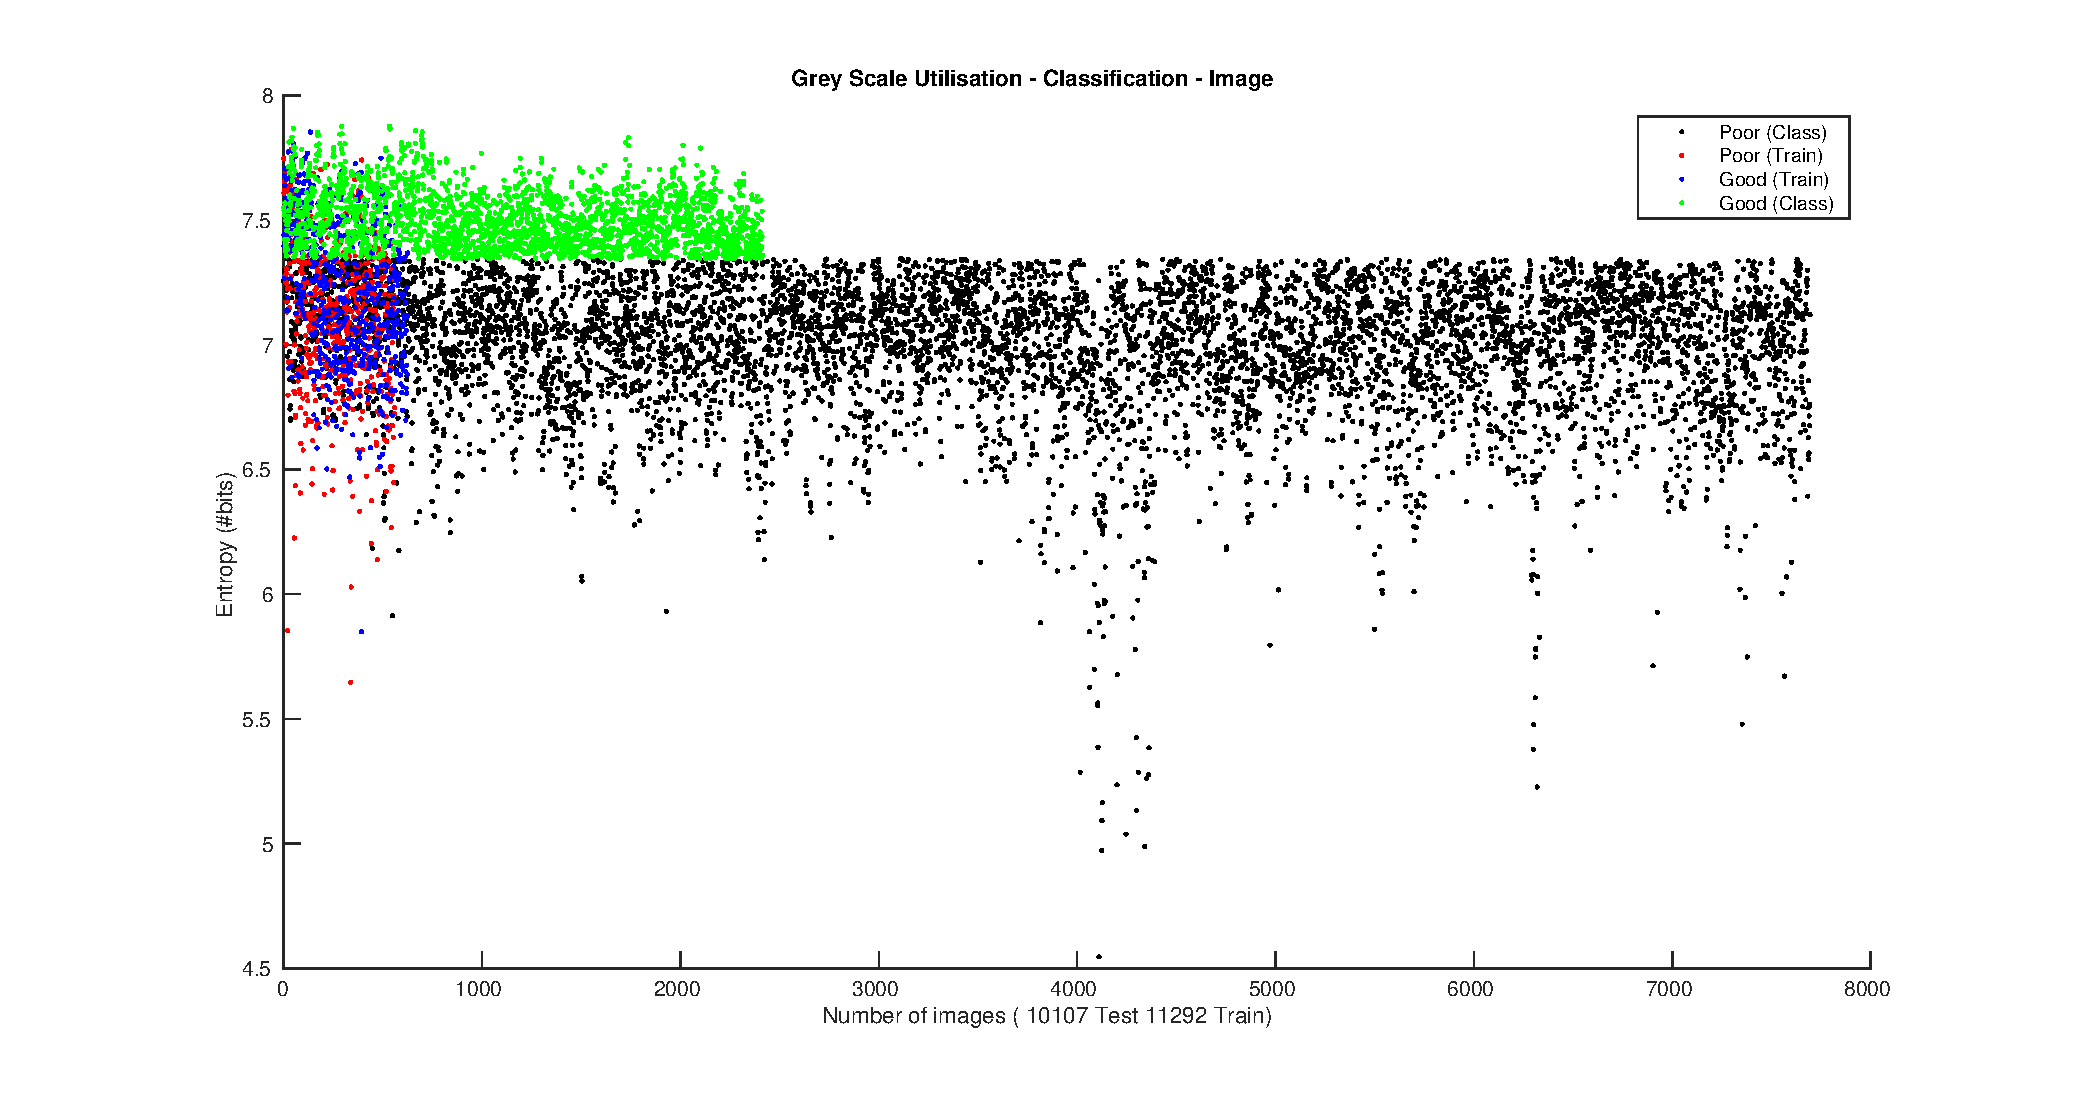
\includegraphics[width=0.9\linewidth, height=1.6cm]{pics/biqa_clas_gsu}
		\caption{Res. of class. using BIQA GSU}
		\label{fig:clas_gsu}
	\end{minipage}
\end{figure}
\begin{figure}
	\begin{minipage}{0.48\linewidth}
		\centering
		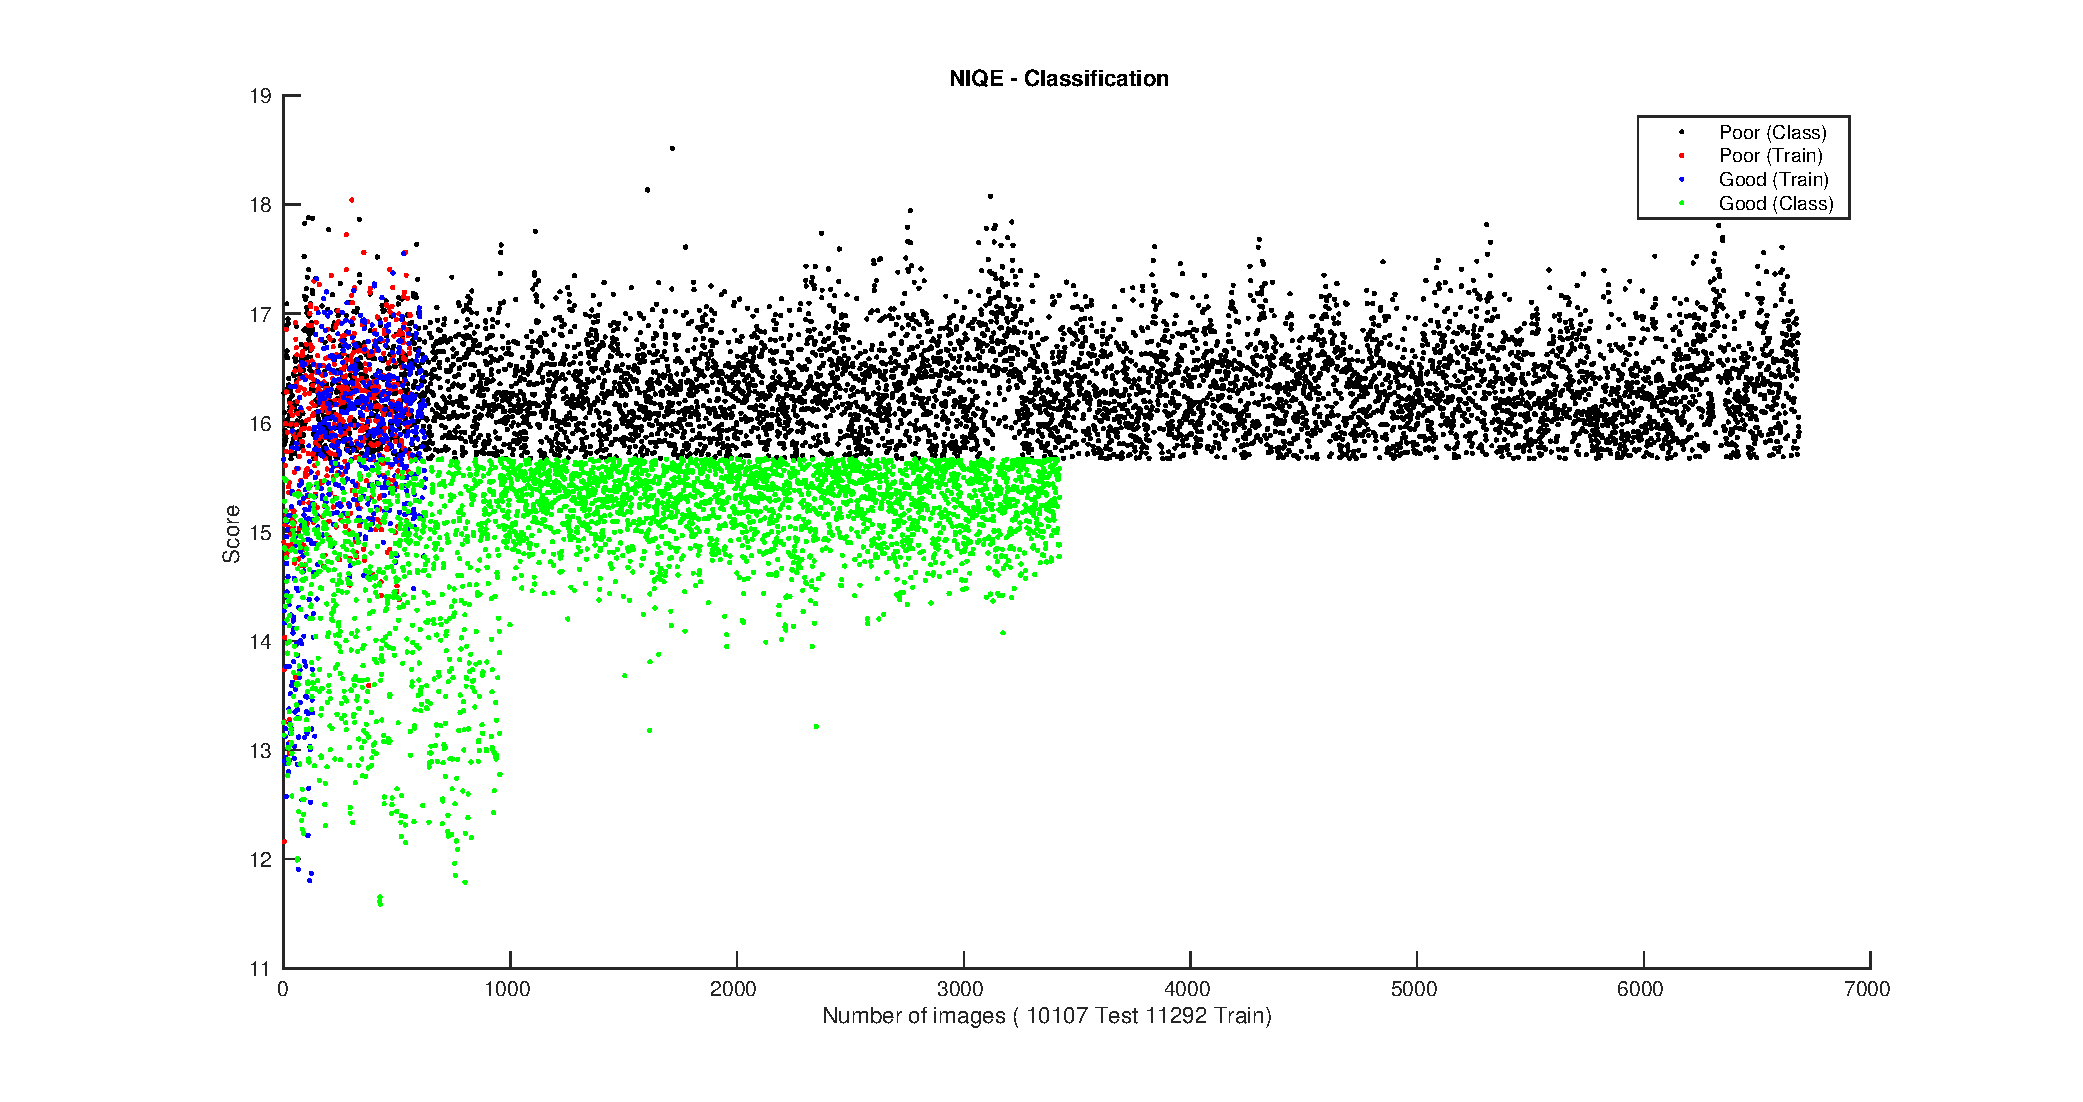
\includegraphics[width=0.9\linewidth, height=1.6cm]{pics/biqa_clas_niqe}
		\caption{Res. of class. using BIQA NIQE}
		\label{fig:clas_niqe}
	\end{minipage}
	\hfill
	\begin{minipage}{0.48\linewidth}
		\centering
		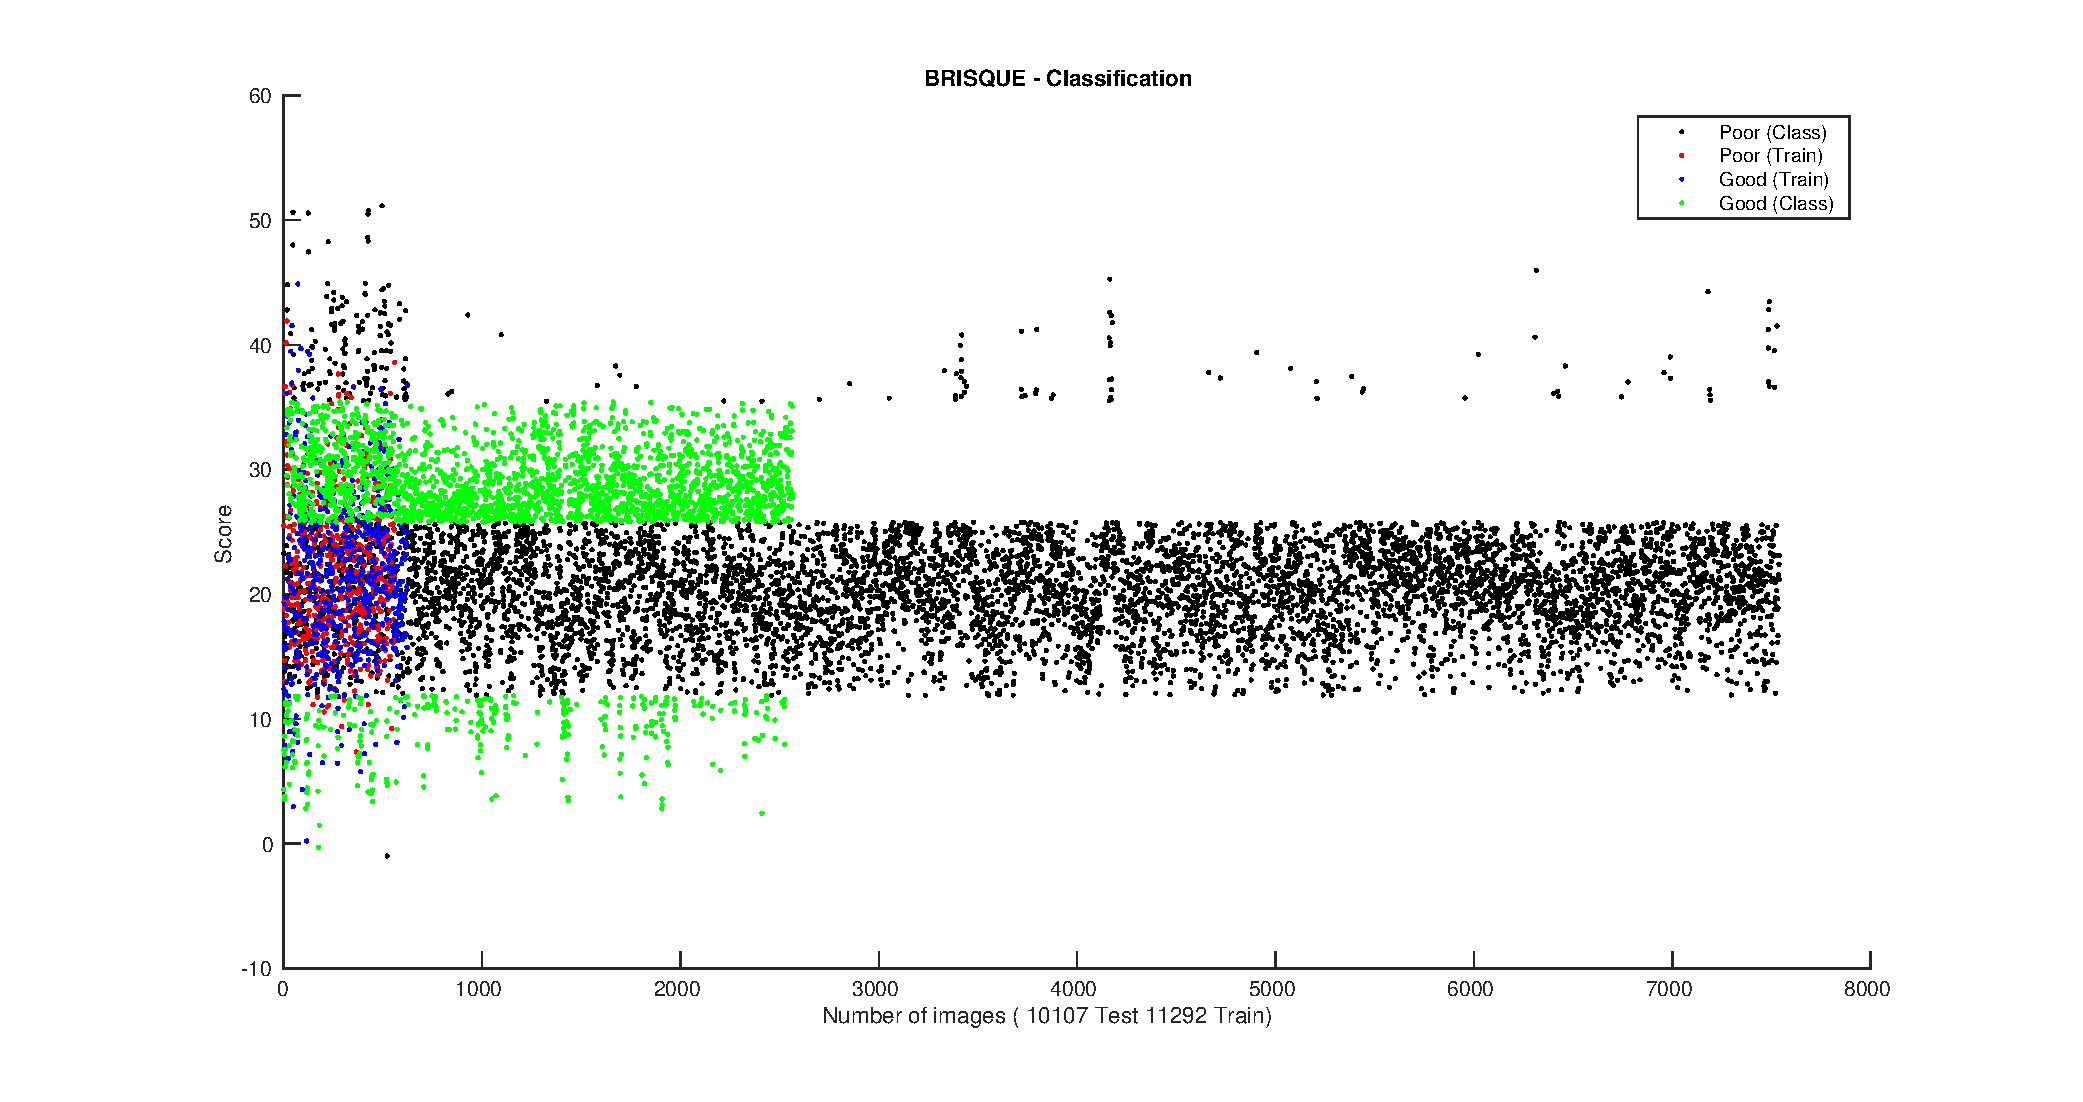
\includegraphics[width=0.9\linewidth, height=1.6cm]{pics/biqa_clas_brisque}
		\caption{Res. of class. using BIQA BRISQUE}
		\label{fig:clas_brisque}
	\end{minipage}
\end{figure}
\begin{figure}
	\begin{minipage}{0.48\linewidth}
		\centering
		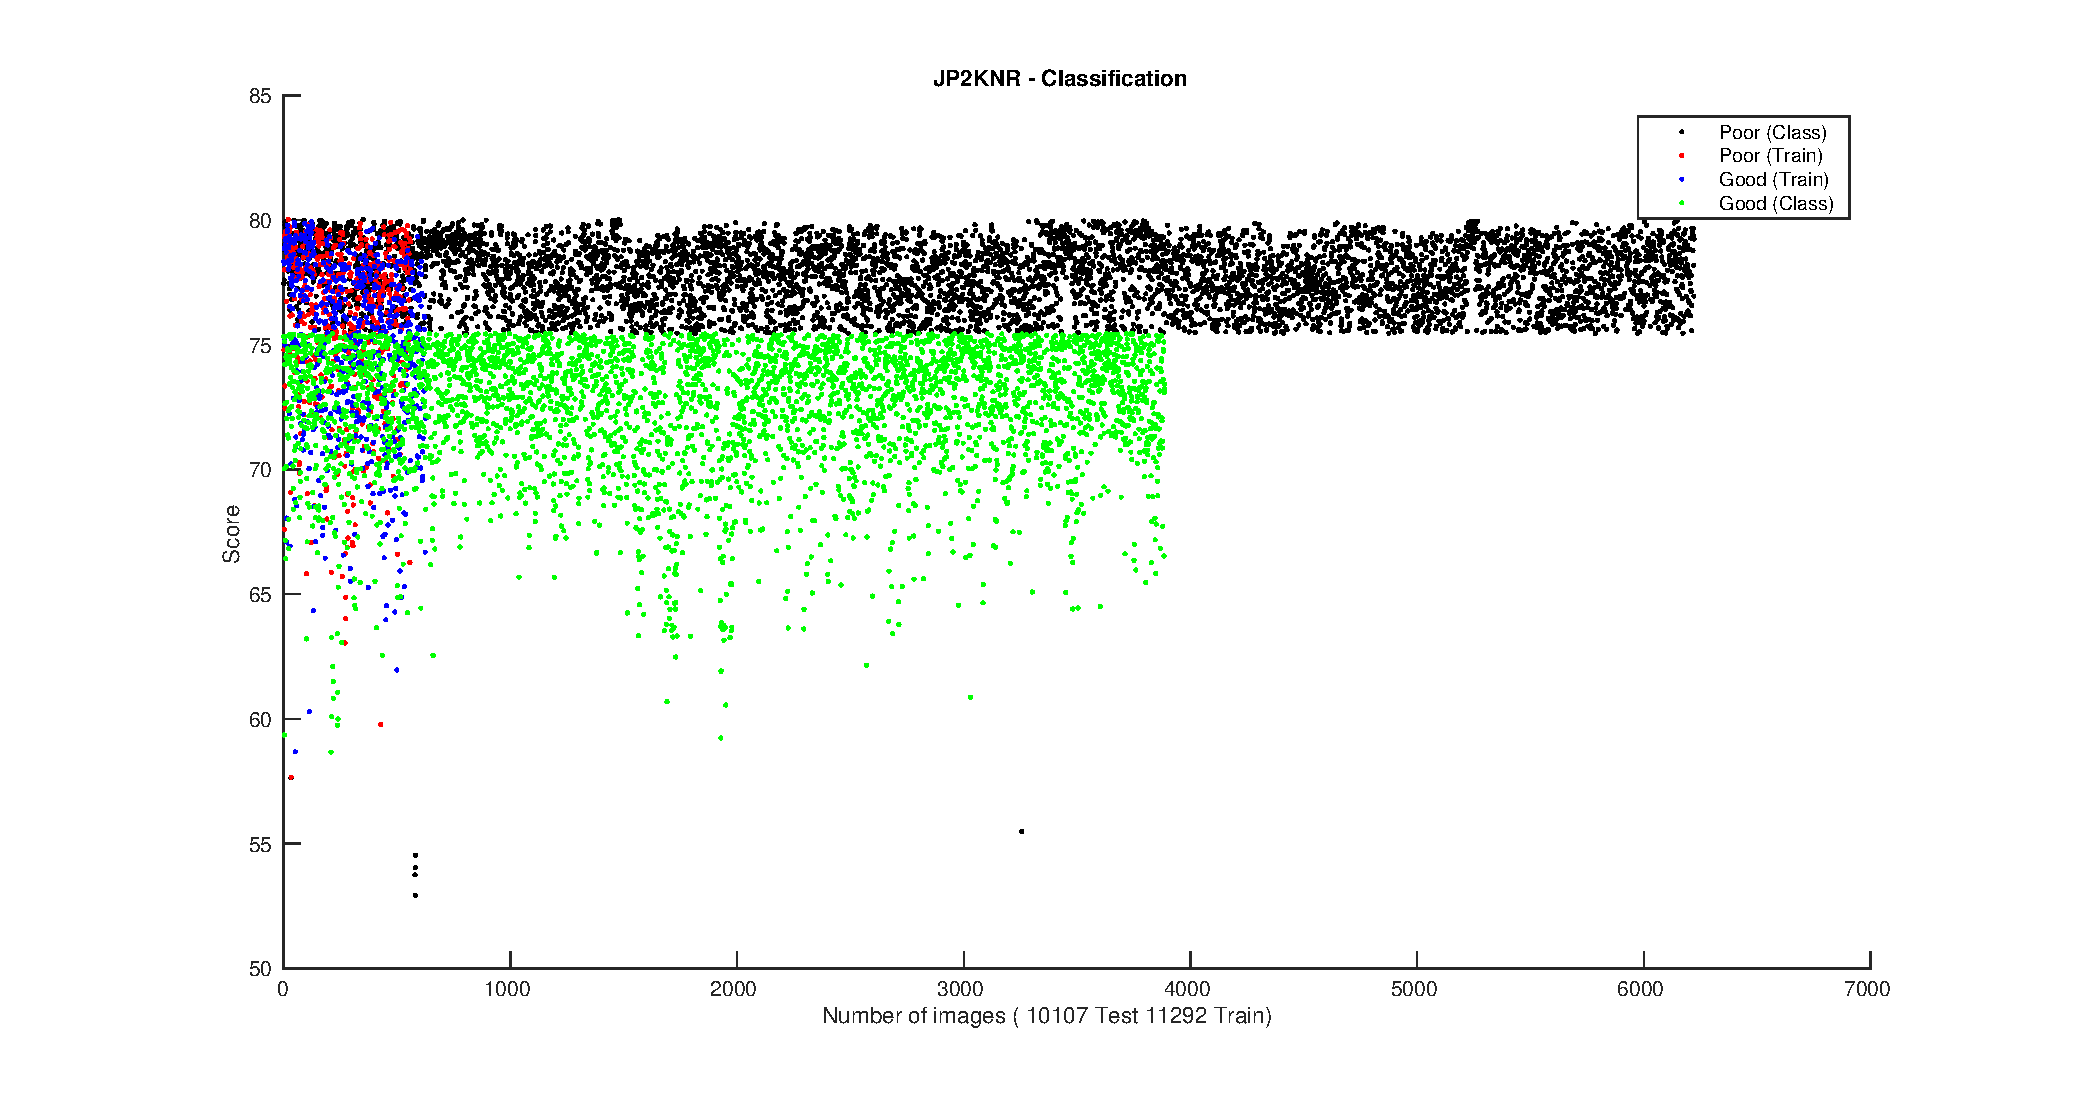
\includegraphics[width=0.9\linewidth, height=1.6cm]{pics/biqa_clas_jp2knr}
		\caption{Res. of class. using BIQA JP2KNR}
		\label{fig:clas_jp2knr}
	\end{minipage}
	\hfill
	\begin{minipage}{0.48\linewidth}
		\centering
		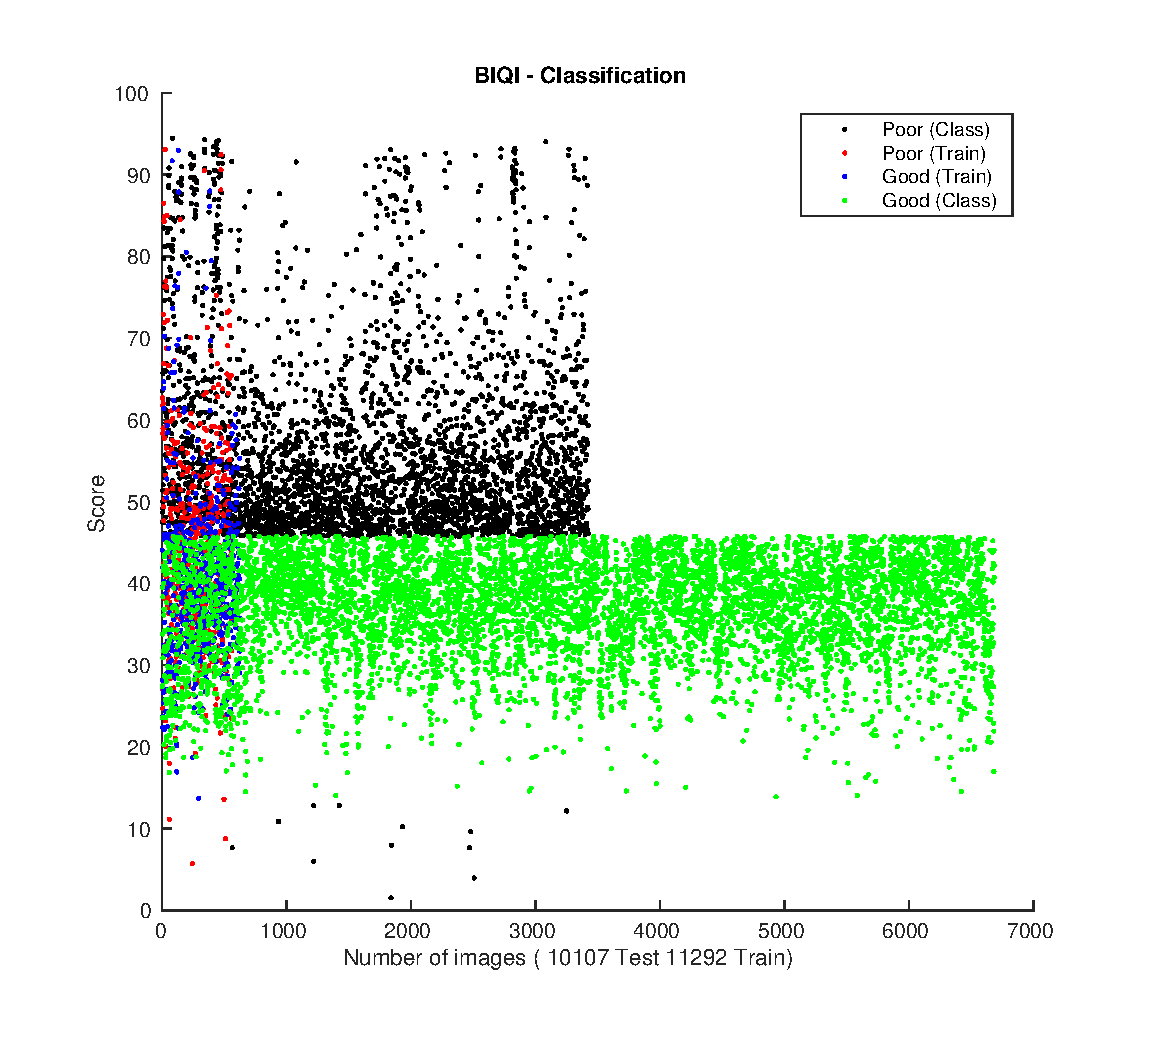
\includegraphics[width=0.9\linewidth, height=1.6cm]{pics/biqa_clas_biqi}
		\caption{Res. of class. using BIQA BIQI}
		\label{fig:clas_biqi}
	\end{minipage}
\end{figure}
\pagebreak
